%auto-ignore
%      this ensures the arxiv doesn't try to start TeXing here.
%!TEX root = super_lattice_models_draft.tex
%      prev line helps TeXShop do the right thing

%%%%%%%%%%%%%%%%
\section{Kitaev wire} \label{kitaev_wire}
%%%%%%%%%%%%%%%%
\ethan{put this as its own section for now, since it's the amalgamation of a bunch of different things. Still undecided about whether this is the best option or not. Maybe putting as an appendix or breaking it up is better}

\dave{Should also cite the two Fidkowski Kitaev papers where they write this wave function down. 
Turzillo et al and Bultinck et al each reiview and extend this work (but that should be double checked).
}
\ethan{cited these papers in the section (only one by fidkowski-kitaev though). Tried to cite them at places where I thought they were relevant, but feel free to change around the citation locations if you disagree}
\dave{I think we still need to do an actual example of the shadow world we explain above. 
This section is very nice for relating the Hamiltonian we define, to the ones that Ware et al, and Tarantino et al define.
}
\dave{
To make this more explicit we can also write the wave function for a single $\beta$ strand embedded in the disk, and do shadow world for that.
}
\ethan{added a short discussion on this at the end, and how it connects with stuff other people have done. Depending on time constraints may or may not want to expand it. I'm good with not making it more verbose, since the actual shadow world 
for the kitaev wire embedded in a 2-manifold is pretty ugly and not too illuminating.}

In this section, we show how the graphical formalism developed in previous sections
can be used to succinctly capture the salient features of the `Kitaev wire', Kitaev's toy model 
of a one-dimensional spinless $p$-wave superconductor \cite{kitaev2001}. 
This elucidates the connection between Majorana zero modes and Ising anyons, serves 
as a nice application of the graphical calculus of the $C_2$ theory, and provides 
a simple (alas, perhaps too simple) illustration of the shadow world approach detailed in the previous section 
(with appropriate modifications for the reduced dimensionality of the problem). 
The Hamiltonian we write down and the associated wavefunctions we construct are 
the same as those found in e.g. \cite{fidkowski2011}, but presented in a more graphical formalism and 
discussed within the framework of the more general tools developed in this paper. 

The Kitaev chain is defined on a one-dimensional manifold, which we can take to be 
either $M = I$, $M= S^1_B$, or $M = S^1_N$, 
where $I$ is an interval. 
The shadow world prescription tells us to examine 
partition functions on $M \times [0,1]$. 
\kw{I'm confused by the dimensions here.  Are we working with a 1+1-dim'l TQFT?  Do you really mean ``partition function"?}
\kw{I guess we can think of this as a dimensional reduction of the C2 theory over an interval $J$ (not to be confused with $M=I$.
This can of course be done for any SPC.} \ethan{I think the philosophy we had (or at least, the one I had) when we wrote this was: ``we construct the Kitaev wire from a physical point of view, not really thinking about dimensional reduction. Then we realize that it's the dimensional reduction of $C_2$ (there's a paragraph on this towards the end of the section), which lets us understand $C_2$ as a bunch of fluctuating Kitaev wires. This connects what we've been doing to other physicist's work.}
We will specify to $M= I$ in what follows, and examine 
chains whose Hilbert spaces contain $N$ tensor factors, where $N=2n$ is an even integer. 
Vectors in $\mch(I)$ can then be written as $a_1\tp\dots\tp a_N$, and graphically 
they look like\footnote{We will be specializing to the case of the $C_2$ theory, and as such we can
refrain from drawing orientations on each edge.}
\dave{Should probably include boundary condition.}
\ethan{you mean tails sticking down, right? If we want to write it as a 1d MPS thing, usually I'd just set them all to the vacuum (which we do in what follows). Can modify the figure and talk about it if you want, though}
\ethan{moved discussion of MPS to the end}
\be  \label{graphical_MPS_state}
\mathord{\vcenter{\hbox{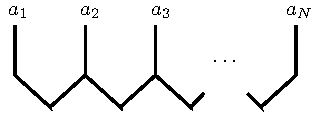
\includegraphics[scale=1]{kitaev_wire_cell_decomp.pdf}}}}.
\ee
For analyzing the Kitaev wire, we will draw the labels $a_i$ from the simple objects of the $C_2$ theory (namely $\unit$ and $\beta$),
and we will freely use 
the graphical calculus of the $C_2$ theory throughout.  
We will see that the $\beta$ object plays the role of a Majorana fermion in the Kitaev wire. 

When performing the shadow world construction, we need to compute partition functions on the 2-manifold 
$M\times [0,1]$. The cell decomposition we will use is:
\dave{boundary condition.}
\be 
\mathord{\vcenter{\hbox{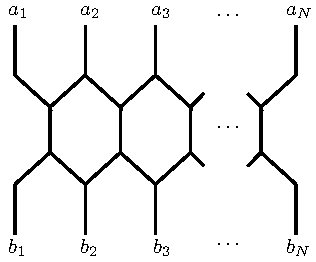
\includegraphics[scale=1]{kitaev_wire_shadow_wrld_cell_decomp.pdf}}}}.
\ee
To construct ground-state wavefunctions, we need to fix the input vectors $v_0\in\mch(M\times\{0\})$ and $v_1\in\mch(M\times\{1\})$ to be used when computing 
$Z(M\times[0,1];v_0,v_1)$. In the above pictures, $v_1$ is determined by the choice of $a_1\tp\dots\tp a_N$, while $v_0$ is determined by the $b_1\tp\dots\tp b_N$. In what follows, 
we will choose $v_0 = \unit\tp\dots\tp\unit$ to be the vector with only vacuum lines, so that our wavefunctions are built
over the vacuum.
% (if we had chosen $\Sigma = S^1_N$ or $S^1_B$, $v_0$ would also need to 
%specify our choice of spin structure). 

Physically, each pair of adjacent tensor factors $a_i\tp a_{i+1}$ forms the Hilbert space of a single 
site in the physical superconductor, so that our $N$-legged chain maps to a superconductor 
with $n=N/2$ physical sites. The degree of freedom living on the $n$th physical site is thus $a_{2n-1}\tp a_{2n}$.  
This association is just the familiar re-writing of a single electronic degree 
of freedom in terms of two Majorana degrees of freedom. 
The local Hilbert space at a given physical site (e.g, at a pair of edges $a_i\tp a_{i+1}$) is $\cc^{1|1}$, and is spanned by the two basis vectors
\begin{align} \label{kitaev_chain_basis_vects}
   v_e = \; \CupSigma \qquad \text{and} \qquad v_o=\;\CupSigmadot.
\end{align}

\dave{Around here I would write out the explicit tensors for the MPS from shadow world.
Then do the following analysis relating to the wave function. 
And finally writing down \eqref{kitaev_wire_ground_states} and saying how it's equivalent to $\ket{\psi} = \sum_{...}\tr (A\cdots) \ket{a_1 \cdots } $. }

\dave{If we're just doing shadow world stuff, we can probably define the Hamiltonian at the very end.}
The Hamiltonian implements time evolution by extending the uncontracted $a_i$ legs on the $M\times\{1\}$ boundary. 
The Hamiltonian must be local, and so it may only act on pairs of adjacent uncontracted legs on the boundary.
The Hamiltonian must also preserve the overall fermion parity of the chain. 
Thus, the only terms one can construct a Hamiltonian out of are
\begin{align} \label{hamiltonian_options}
\Id \qquad \text{and} \qquad \TwoLinedotdot.
\end{align}
The first is the identity operator, while the second is nontrivial and is identified with $i \gamma_1 \gamma_2$, 
a Majorana bilinear which acts as the fermion parity operator $(-1)^F$ on the on-site Hilbert space.
To see this, we can simply check the action of the second term on the basis vectors of the single (physical) site Hilbert space. 
Graphically, the  
second term acts by stacking diagrams onto input states, and so it acts
on single-site basis states as
\begin{align}
\TwoLinedotdot\; \circ \; \CupSigma \; =\;  \CupSigma \quad \text{and} \quad \TwoLinedotdot\; \circ\; \CupSigmadot \; =\;   - \; \CupSigmadot.
\end{align}
This is precisely the action of the Majorana bilinear $i\gamma_1\gamma_2 = (-1)^F$, 
and we will build the Hamiltonian out of a summation of such terms. 

\ethan{maybe move this to a reflection / inner product section if it gets written, although I think the 
stuff in the line bundle appendix is sufficient if we're short on time}
In order to show that this term is Hermitian, we need to define a graphical way of implementing 
Hermitian conjugation. We define the Hermitian conjugate of a diagram to be its reflection about 
the horizontal axis, with the action of reflection determined by the properties of the complex line 
bundle constructed in Appendix \ref{flb_appendix}. One then verifies that $H^\dagger H = -\lambda^2 \unit$, where the 
minus sign is a Koszul sign, $\lambda$ is the phase picked up when removing a pair of fermions 
as in \eqref{removing_fermions}, and $\unit$ denotes a sum of identity operators (the left picture in \eqref{hamiltonian_options}). 
As usual, the notation $H^\dagger H$ graphically corresponds to stacking $H^\dagger$ on top of $H$.
Since $\lambda^2 = -1$ as we prove in Appendix \ref{fib_appendix}, we verify that $H^\dagger H = \unit$.  

For our $N$-legged chain we thus have the basis of states $\bigotimes_{i=1}^{N/2} v_i$, where 
$v_i \in \{v_e,v_o\}$ are $\pm1$ eigenstates of $(-1)^F$. 
Graphically, these states look like
\begin{align}
&\CupSigma \; \CupSigma \; \CupSigma \cdots \CupSigma,\\
&\CupSigmadot \; \CupSigma \; \CupSigma \cdots \CupSigma,\\
&\CupSigma \; \CupSigmadot \; \CupSigma \cdots \CupSigma,\\
&\CupSigma \; \CupSigma \; \CupSigmadot \cdots \CupSigma,\\
&\CupSigma \; \CupSigma \; \CupSigma \cdots \CupSigmadot,\\
&\CupSigmadot \; \CupSigmadot \; \CupSigma \cdots \CupSigma,
\end{align}
and so on. In the above picture, there are $n=N/2$ cups appearing, and the fermion dots are ordered 
implicitly with increasing Koszul ordering from left to right. 

The Hamiltonian, built out of the identity and the bilinears $i\gamma_1\gamma_2$, has two types of terms. 
One term mixes the states within a single physical site by acting on $a_{2j}\tp a_{2j+1}$, while the other acts between neighboring physical sites by acting on 
$a_{2j+1}\tp a_{2j+2}$.
We will denote the former terms by $H_{2j}$ and the latter terms by $H_{2j+1}$.
Then the Hamiltonian takes on the form
\begin{align}
H = - \sum_{j=1}^{N-1}\;  \frac{t_j}{2} \left( \Id_{\text{\; site $j$}} \;\; + \;\; \TwoLinedotdot_{\text{site $j$}} \right),
\end{align}
where the left lines are applied to site $j$ and the right line is applied to site $j+1$.
\ethan{I am in favor of writing the Hamiltonian like this, with the understanding that when we draw pictures and stuff, we are modding out by fermion slides and that the spin framing is fixed so that we have the usual $C_2$ diagrammatic manipulations. We can talk about $\alpha(e)$ stuff and edge terms to implement endos etc, but I think we probably shouldn't}

To study the Kitaev wire in its topological phase, we will work in the completely staggered limit, where
the inter-site terms $H_{2j+1}$ dominate and the intra-site terms $H_{2j}$ are absent\footnote{Physically, this corresponds to tuning the chemical potential to zero and the 
magnitude of the superconducting gap to the hopping amplitude.}, 
so that the Hamiltonian is 
\begin{align} \label{staggered_H}
H_{\rm staggered} = - \sum_{j=1}^{n-1}\; \frac{1}{2} \left( \Id_{\text{\; site $2j$}} \;\; + \;\; \TwoLinedotdot_{\text{site $2j$}} \right),
\end{align}
where we have set the hopping strength to $1$ for simplicity. Note that in this form, the Hamiltonian 
is a projector. 
In this limit the wire is in the topological phase and there are two zero-energy ground states, differing by their fermion parity:
%\dave{Maybe we should also change basis so that we see that the wave function is a coherent sum over all parity even (odd) states.}
\begin{align} \label{kitaev_wire_ground_states}
\Psi_e = \;\StaggaredGSEven \; \cdots \; \StaggaredGSEvenR\;, 
\qquad \text{and} \qquad 
\Psi_o =\; \StaggaredGSOdd \; \cdots  \; \StaggaredGSEvenR.
\end{align}
To better understand these wavefunctions, we can perform a change of basis by applying $F$-moves to 
each cup-cap pair with the $F$-move \eqref{cupcap_fmove}. 
On a Kitaev wire with $n$ physical sites, we have
\be \Psi_e = \frac{1}{d^{n-1}} \bigotimes_{i=1}^n (-A^4)^{n_f/2} \sum_{\{v_i\}}  v_i,\ee
where the sum is over all combinations of $v_i =v_o,v_e$ such that only an even number $n_f$ of $v_o$ vectors appear 
in the tensor product, and where $v_e,v_o$ are defined as in \eqref{kitaev_chain_basis_vects}.
For the odd wavefunction $\Psi_o$, we get 
\be \Psi_e = \frac{1}{d^{n-1}} \bigotimes_{i=1}^n(-A^4)^{(n_f+1)/2} \sum_{\{v_i\}}  v_i,\ee
where the sum is now restricted so that only an odd number $n_f$ of $v_o$ vectors appear 
in the tensor product.
From the expressions for $\Psi_e,\Psi_o$ in this basis, we see that they are given by configurations 
that are coherent sums over all fermion parity even and fermion parity odd states, respectively.  

Note that the fermion dot appearing in $\Psi_o$ has zero energy, while this is not true for fermion dots 
on the interior intermediate cups.
Physically, this implies the presence of two Majorana zero modes, which are identified with the $\beta$ 
lines $a_1,a_N$ at the ends of the chain which are not acted on by the staggered Hamiltonian \eqref{staggered_H}. 
Excited states are easily constructed by putting dots on the intermediate cups. 

A nice feature of our diagrammatic notation is that the ``delocalization" of the fermion number in the topological phase of the 
Kitaev wire is made manifest.
For example, the fermion in the odd-parity state $\Psi_o$ is not localized: it is free to slide along the bottom $\beta$ line
from one end of the chain to the other (with the sliding being implemented through the odd elements in $\End(\beta)$
as usual).

If we instead consider the Kitaev chain on a circle, the wavefunctions can be found in a similar manner, 
namely by computing partition functions of the form $Z(S^1_X;v_0,v_1)$, where $X\in\{B,N\}$
specifies the choice of spin structure. 
If we again set the input state to be $v_0=\unit\tp\dots\tp\unit$, the graphical depiction of the 
ground-state wavefunctions 
has a similar form to those in \eqref{kitaev_wire_ground_states}, except the bottom $\beta$ string 
forms a closed loop below the series of $\beta$ cups. 
In this case, the fermion parity of the wavefunction is uniquely determined by the spin structure, being 
even for $S^1_B$ and odd for $S^1_N$, which can be verified using the graphical calculus for the 
$C_2$ theory. For both spin structures, the ground state is unique. 
The odd-parity $S^1_N$ wavefunction hosts a single fermion dot on the lower circular $\beta$ line, 
and the delocalization of fermion parity is again manifest, as the exact location of the fermion dot 
is arbitrary. 

Note that the way we draw vectors in the Hilbert space of the Kitaev wire \eqref{graphical_MPS_state}
is just a graphical presentation of a matrix product state (MPS), with the labels
$a_1,\dots,a_N$ constituting the physical indices and the unlabeled (contracted) edges hosting the virtual 
indices (which are also drawn from the label set $\{\unit, \beta\}$). 
In the MPS formalism, a vertex on which the leg labeled $a_i$ is attached 
to is associated with a matrix $A^{a_i}_{xy}$, where $x,y$ are virtual indices. 
The $A^{a_i}$ matrices can be determined from the shadow world approach 
discussed above, and in this case are given by the structure constants of $\cliff_1$ \cite{turzillo2016}. 
Wavefunctions are then constructed by contracting the virtual indices following the 
shadow world prescription. To construct a wavefunction $|\Psi\rangle$ we need to compute 
partition functions of the form $Z(M;\emptyset,v_1)$, where $\emptyset$ denotes 
the input vacuum state. 
By using our earlier results \eqref{bounding_trace} and \eqref{nonbounding_trace} on 
partition functions, we see that 
\be |\Psi\rangle = \sum_{\{ a_i \} }\tr(A^{a_1} \cdots A^{a_N}) \ket{a_1 \cdots a_n} \ee
if the Kitaev wire is defined over an interval or on $S^1_B$, and 
\begin{align}
 |\Psi\rangle & = \sum_{\{ a_i \} }\tr((-1)^FA^{a_1} \cdots A^{a_N}) \ket{a_1 \cdots a_n} \\ 
 & =\sum_{\{ a_i \} }\str(A^{a_1} \cdots A^{a_N}) \ket{a_1 \cdots a_n} 
 \end{align}
if the wire is defined on $S^1_N$. 
This is the presentation of the wavefunctions used in the tensor network community, 
and agrees with the results of \cite{turzillo2016,bultinck2017b}. \ethan{other references?}

\ethan{for some reason I can't write this well---maybe Dave can do better}
This $(1+1)$-dimensional example sheds some light on the $(2+1)$-dimensional examples 
considered in the majority of the paper. For example, in the simple case of the $C_2$ theory, 
$\beta$ strings are equivalent to fluctuating Kitaev chains in their topological phase. 
We can see this by considering a state in the $C_2$ theory constructed 
from the shadow world approach with $v_0 = \emptyset$ and $v_1$ a state 
with a single $\beta$ loop which inherits spin structure $X$. 
The degrees of freedom in this state are the same as 
the degrees of freedom in the Kitaev chain constructed over $S^1_X$, 
where we identify each vertex Hilbert space with a pair $a_{2j}\tp a_{2j+1}$ of Majoranna
variables connecting two adjacent physical sites. 
Furthermore, the Hamiltonian defined in Section \ref{Super_pivotal_Hamiltonian} is the same as the Kitaev 
chain Hamiltonian \eqref{staggered_H} when acting on $v_1$. 
The vertex and plaquette terms are trivially satisfied by the choice of $v_1$, and so we only need to focus 
on the edge term $\lambda_e \sum_{e\in \mce} (1-D_e)$. As described in Section \ref{edge_term}, 
the operator $D_e$ changes the fermion parity of the vertices $v,v'$ at the ends of the edge $e$, provided
that $e$ is colored by a $\beta$ line. 
This is exactly the same process implemented by the Kitaev wire Hamiltonian: both Hamiltonians
 are responsible for ``sliding'' fermions along $\beta$ strings.  

To summarize, states in the $C_2$ theory are formed from superpositions of fluctuating Kitaev chains, which in our case are exactly equivalent to $\beta$ strings. 
With these remarks in mind, it 
is natural to view q-type strings in more general $(2+1)$-dimensional super fusion categories 
as different types of fluctuating Kitaev chains, which is a point of view adopted in\cite{tarantino2016,ware2016,kapustin2017}. 
There are several pieces of evidence for this: the fermion parity of a closed q-type string 
depends only on the string's homology class and is determined by the spin structure it inherits, 
and in the simplest case of the $C_2$ theory, q-type strings literally are Kitaev chains, as shown 
above. 

However, we have seen examples of theories in which q-type strings do not behave like Kitaev wires.
In such theories (like the $SO(3)_6$ and $\halfesix$ examples considered earlier), two q-type
strings can fuse to a q-type string, and two m-type strings can fuse to a q-type. 
If all open q-type strings hosted Majorana zero modes at their ends, such fusion rules would 
be disallowed, since the number of Majorana zero modes must be preserved modulo 2. \ethan{do we even want to mention the above paragraph? More importantly, is it correct? Dave probably knows this best}




%When transforming back to the original basis, one sees that the state is actually an even superposition of all possible placements of an even number of fermions, similarly for the odd state.


 
 